\chapter{PRE \Author{F. Chow, J. Knoop and O. R\"uthing}}
\inputprogress
\graphicspath{{img/}{pre_not_helped/img/}{part3/pre_not_helped/img/}}
\chapterauthor{F. Chow, J. Knoop and O. R\"uthing}

\section{Introduction}

Redundancy elimination is an 
important category of optimizations performed by modern optimizing compilers.
In the course of program execution, certain computations may be repeated
multiple times that yield the same values.  Such redundant
computations can be eliminated by saving the results of the earlier 
computations for reuse later.  

There are two types of redundancies: \emph{full} redundancy and 
\emph{partial} redundancy.  A computation is fully redundant if the 
computation has occurred earlier regardless of the flow of control.
The elimination of full redundancy is also called common subexpression
elimination, and if applied at the global scope, it is called global common
subexpression.  A computation is partially redundant if the computation has
occurred earlier only on some paths of execution, and where there is at
least one control flow path where that computation has not occurred earlier.

There are two different methods to identify whether two computations are the 
same: the \emph{lexical} method and the \emph{semantic} method.  The 
lexical method applies to expressions that are lexically identified.
Under the lexical method, two computations are the same if they
are written the same way using variables and/or constants before conerting
to SSA, like $a+3$.  In this case, redundancy can come up only if the 
variables' values have not changed between two occurrences.
The semantic method applies to computations based on operands that are
not necessarily identical by name, but known to have the same values.
For example, $a+b$ and $a+c$ will compute to the same result
if $b$ and $c$ are known to hold the same value.
In this chapter, we are mostly dealing with lexically identified
expressions.  Section~\ref{section:Part3:Pre_not_helped:SemanticPRE} will
address redundancy elimination among computations that yield the same value.

The concept of partial redundancy was originally introduced by Morel and 
Renvoise \cite{MR79}.  Before the technique of partial redundancy 
elimination was developed, optimizing compilers have been performing
global common subexpression elimination and loop invariant code motion in
separate global optimization phases.  Morel and Renvoise showed that
global common subexpressions and loop-invariant computations are special
cases of partial redundancies, and can be subsumed by partial redundancy
elimination (PRE).  Morel and Renvoise formulated PRE as a code placement
optimization problem, in which additional computations will be inserted at
certain points in the program.  Such insertions make the original
partially redundant computation become fully redundant, and so can be
trivially deleted.  The PRE algorithm developed by Morel and Renvoise
involves bi-directional data flow analysis, which incurs more overhead
than uni-directional data flow analysis.  In addition, their algorithm
does not yield optimal results in certain situations.

An alternative placement strategy, called lazy code motion (LCM), was later 
developed by Knoop {\it et al.} \cite{Knoop92}\cite{Knoop94}.  It improves on
Morel and Renvoise's results by avoiding unnecessary code movements and by
removing the bi-directional nature of the original PRE data flow equations.
The results of lazy code motion is optimal: the number of computations cannot
be further reduced by \emph{safe} code motion \cite{Kennedy72}, and the
lifetimes of the temporaries introduced for storing the computed values
are minimized.

The above approaches to PRE are all based on a bit-vector formulation of the
problem and on the iterative solution of data flow equations.
The use of SSA to solve PRE was proposed by Chow {\it et al.} 
\cite{Chow97}\cite{Kennedy99}.  Their SSAPRE algorithm is an adaptation of LCM
to SSA.  It represents the first use of SSA to solve data flow problems
related to expressions in the program.  The SSAPRE algorithm brings all
the desirable characteristics of SSA to PRE, and represents a further
refinement to solving PRE.  SSAPRE does not involve traditional iterative
data flow analysis in its solution.  It takes advantage of the \emph{sparse}
representation of SSA, where information associated with an object is
represented only at places where it changes, or at its actual occurrences
in the program.  Sparse representations incur less representation
overhead by avoiding needless duplication of data.  Information can be
propagated through a sparse representation in a smaller number of steps
than through a dense structure, speeding up the algorithms.  By giving up
the use of bit vectors, it sacrifices the parallel solution of bit vectors
in which all program expressions are operated on simultaneously.  But working
on each expression separately has its own advantage in being able to
customize the optimization application on an individual basis.

Another advantage of using SSA is that we do not have to implement the local
and global versions of the optimization separately.  Within a basic block,
the absence of branches guarantees that only full redundancy can be present.
PRE via traditional bit-vector-based data flow analysis only covers global
redundancies.  A separate algorithm needs to be implemented to recognize
local common subexpressions.  In contrast, the SSAPRE algorithm uniformly
covers both local and global redundancies.

SSAPRE exploits the use-def information built into the SSA form.  It saves
the overhead of having to scan the contents of each basic block in the
program to initialize the bit vectors.  A program transformation that
destroys SSA would require a post-pass to fix the SSA form.  In contrast,
SSAPRE maintains the entire program in valid SSA form throughout,
thus saving the overhead of having to run any SSA fix-up pass.

The rest of this chapter is organized as follows.  Section 2 describes
the basics of PRE and explains why PRE and SSA are related.
Section 3 describes the SSAPRE altorithm.
Section 4 discusses some issues related to the practical implementation 
of SSAPRE.
Section 5 discusses how SSAPRE can be made to perform speculation.
Section 6 describes applying PRE to perform register promotion.
Finally, Section 7 discusses redundancy under the semantic approach.

\section{Why PRE and SSA are related}
\label{section:Part3:Pre_not_helped:PRErelatedtoSSA}

A partially redundant computation is a computation that is redundant in
some path of execution.  In Figure~\ref{fig: pre-examples}(a), the
computation $a+b$ is redundant when the right path is taken.
In Figure~\ref{fig: pre-examples}(b), the $a+b$ is redundant whenever
the branch-back edge of the loop is taken.
Partial redundancy elimination can be thought of as a two-step process.
The first step involves deciding where to insert the computation so as to
render the partially redundant computation fully redundant.  The second
step then delete the fully redundant computation.  Since the second step is
trivial and well understood, the main challenge lies in the first step
for coming up with the best set of insertion points.

\begin{figure}
\centering
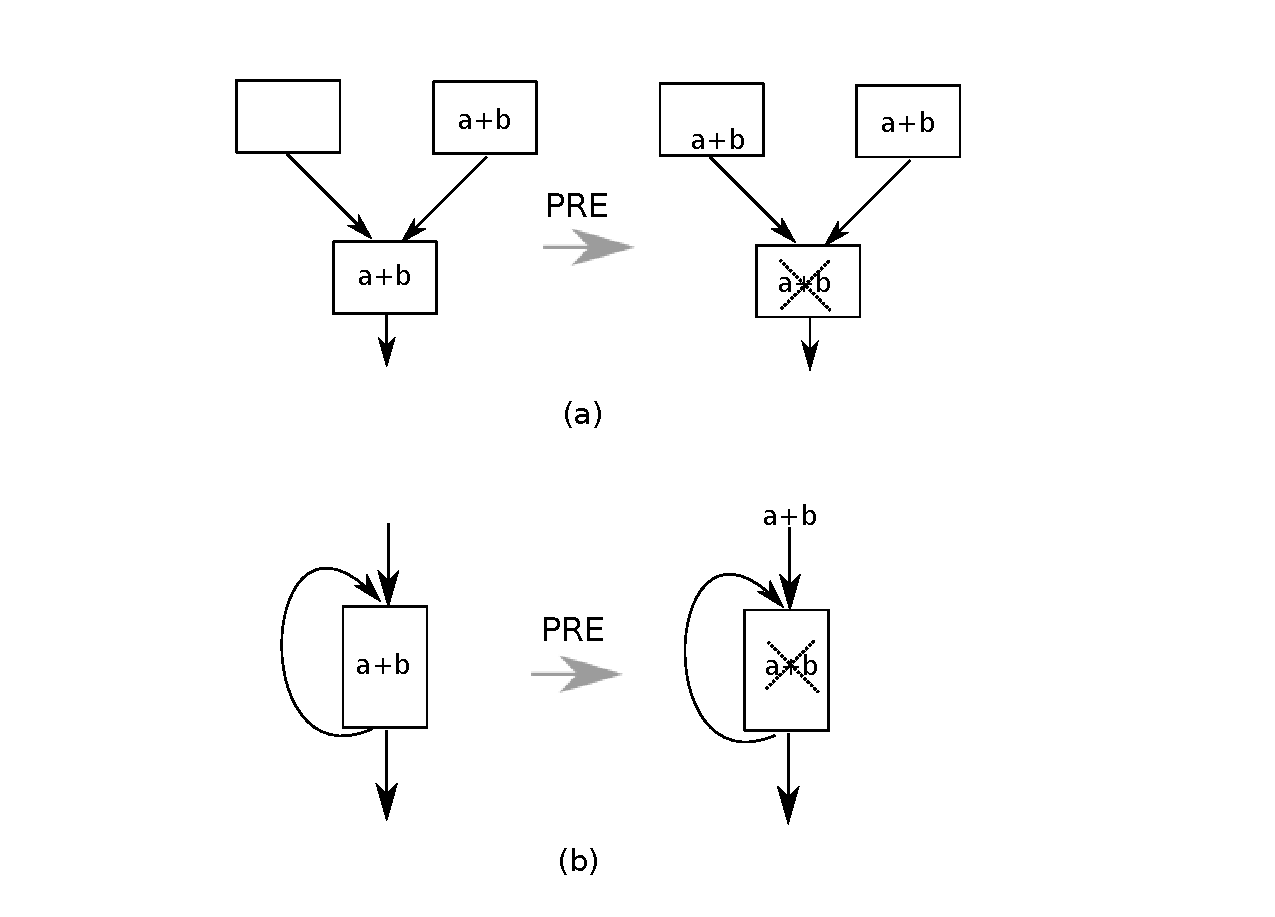
\includegraphics[scale=0.45]{fig-pre-examples.pdf}
\caption{Two basic examples of partial redundancy elimination.}
\label{fig: pre-examples}
\end{figure}

Since there has to be insertion in order to eliminate each partial
redundancy, we can visualize the impact on redundancies of a computation
in the control flow graph.  As illustriated in
Figure~\ref{fig: ssapre-motive}, in the region that is dominated by the 
computation, any further occurrence of the same computation is fully 
redundant.  Once we are past the dominance frontiers, any occurrence is
partially redundant.  In constructing SSA form, dominance frontiers are where
$\phi$'s are inserted.  And since $\phi$ is the key ingredient of SSA, we
can see that PRE is in fact related to SSA, in the sense that finding where
to do insertion in PRE is analogous to finding where to insert $\phi$'s in
constructing SSA form.

We use the term \emph{placement} to refer to the set of points in the 
optimized program where a particular computation occurs.
As we mentioned earlier, SSAPRE works on one computation at a time.
Given a lexically identified expression, e.g. $a+b$, SSAPRE will find
a placement that satisfy the following three requirements in this order:
\begin{enumerate}
\item All inserted computations are \emph{safe}.  This means that no new 
computation will be introduced to any path in the program that did not 
origianlly contain the computation.  This requirement prevents incorrect 
behavior of the optimized program in the presence of computations that may 
cause exceptions.
\item The placement is \emph{computationally optimal}.  This means that no
other safe placement can result in fewer occurrences of the computation
along any path from entry to exit in the program.
\item The temporaries introduced to store the computations for reuse in the
computationally optimal placement are life-time optimal.  This means that
for the purpose of allocating the temporaries to registers, it will not
induce more register pressure than needed.
\end{enumerate}

\begin{figure}
\centering
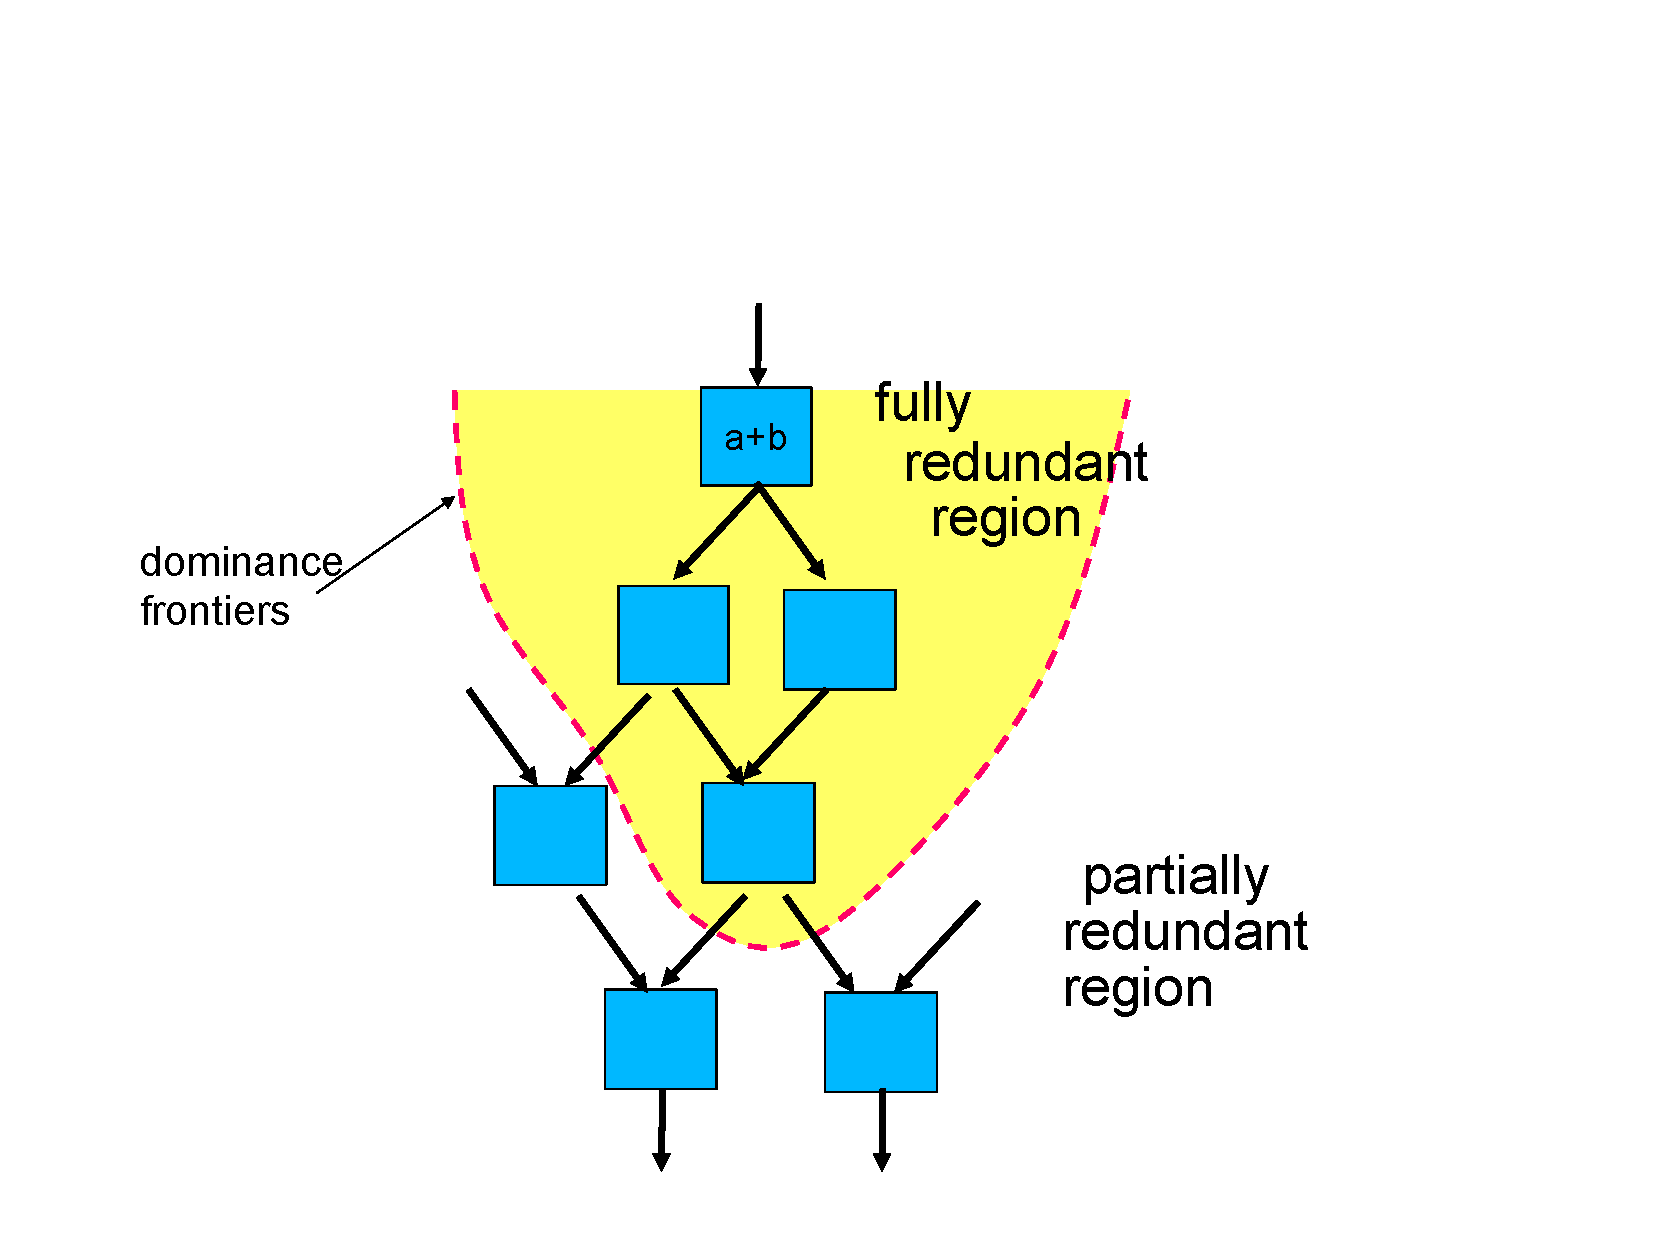
\includegraphics[scale=0.35]{fig-ssapre-motive.pdf}
\caption{Dominance frontiers are boundaries between fully and partially redundant regions.}
\label{fig: ssapre-motive}
\end{figure}

Since avoiding redundant computation requires saving the values of 
computations into temporaries and re-using their values later, this is
analogous to modeling the flow of data values in variables using SSA form.
The PRE problem can be viewed as determing the best way to store and
reuse a given computation.  Thus, we can visualize this problem using
the temporary that will be used for that purpose.  This is a superset of
the problem of constructing SSA form for a program variable, because,
in addition of putting the temporary into SSA form, 
we determine new placements for the computation and also determine
which occurrences are defs and which occurrences are uses.  In fact, the
SSAPRE algorithm can be regarded as a not-so-trivial extension of the SSA 
construction algorithm, as we'll see in the next section.

\section{The SSAPRE Algorithm}

We assume the input program is already in SSA form.  We also assume 
the dominator tree (DT) and iterated dominance frontiers (DF$^+$) with
respect to the control flow graph of the program are also available, since
they must have been computed for putting the program into SSA form.
To make the algorithm simpler, we also assume that all \emph{critical edges}
in the control flow graph have been removed by inserting empty basic blocks
at such edges\footnote{A critical edge is one whose tail block has multiple
successors and whose head block has multiple predecessors.}\cite{Rosen88}.
This allows us to model insertions as edge placements, even though we only
insert at the ends of the predecessor blocks.

We also make the following two simplifying assumptions about the input SSA
form:
\begin{enumerate}
\item Each $\phi$ assignment has the property that its left-hand-side and
all of its operands are versions of the same variable; and
\item The live ranges of different versions of the same variable do not
overlap.
\end{enumerate}

In the algorithm description, we assume we are working on an expression like
$a+b$ whose computed values are going to be stored in the hypothetical
temporary $h$.  Since the SSA construction for $h$ is on top of the program
that is already in SSA form, we use upper case $\Phi$ in $h$'s SSA form to 
contrast it with the $\phi$'s that are in the original program.

SSAPRE consists of six separate steps: (1) $\Phi$-Insertion, (2) Rename,
(3) DownSafety, (4) WillBeAvail, (5) Finalize and (b) CodeMotion.
$\Phi$-Insertion and Rename are the SSA construction steps for $h$.  They
correspond to the two steps in the SSA construction algorithm, with 
extensions to deal with situations that apply only to expressions.  After
the Rename step, occurrences of $a+b$ that are assigned the same version
of $h$ must compute the same value.  At this stage, the points of defs and
uses of $h$ have not yet been determined.  Many $\Phi$'s inserted for $h$
are also unnecessary.  Later steps in SSAPRE will fix them up.  Some $\Phi$
operands can be determined to be undefined ($\bot$) after Rename because 
there is no available computation of $a+b$.  These $\bot$-valued
$\Phi$ operands will play a key role in the later steps of SSAPRE because
insertions are performed only because of them.  We call the SSA graph for
$h$ after Rename the \emph{dense SSA graph} because it contains more $\Phi$'s
than in the minimal SSA form.

The sparse computation of global data flow attributes for $a+b$ will be
performed on the dense SSA graph for $h$ in the DownSafety and WillBeAvail
steps.  These analyses only need to focus on the $\Phi$'s, because they
are the only candidates for inserting the expression.
The DownSafety step performs backward propagation to determine 
the $\Phi$'s whose results are not fully anticipated with respect to 
$a+b$.  The WillBeAvail step performs forward propagation to determine
the $\Phi$'s where the computation of $a+b$ will be available assuming
PRE insertions have been performed at the appropriate incoming edges of the
$\Phi$'s.  At this point, using the results of the data flow analysis, we
are ready to finalize the effects of PRE.  The Finalize step inserts
computation of $a+b$ at the incoming edges of $\Phi$ to ensure that the
computation is available at the merge point.  For each occurrence of 
$a+b$, it determines if it is a def or use of $h$.  It also links the
uses of $h$ to their defs to form its \emph{precise SSA graph}.
Extraneous $\Phi$'s are removed so that $h$ is in minimal SSA form.

The last CodeMotion step updates the program to effect the code motion for
$a+b$ as determined by SSAPRE.  It introduces the real variable $t$
to eliminate any redundant computations of $a+b$.  The $\Phi$'s for $h$
are translated into $\phi$'s for $t$ in the native SSA form of the
program.

We now describes the six steps of SSAPRE in more detail.

\subsection{Step 1: $\Phi$-Insertion}

A $\Phi$ for an expression is needed whenever different values of the
expression reach a common point in the program.  There are two different
situations for this to occur:

First, when an expression appears, we insert a $\Phi$ at its iterated
dominance frontiers, because the occurrence may corespond to a def of $h$.
This is the situation in Figure~\ref{fig: phi-insertion}(a).

The second situation that causes insertion of $\Phi$'s is when there is a
$\phi$ for a variable contained in the expression, because such a $\phi$
indicates that an alteration of the expression reaches the merge point.
In Figure~\ref{fig: phi-insertion}(b), the $\Phi$ at block 3 is caused by
the $\phi$ for $a$ in the same block, which in turns reflects the
assignment to $a$ in block 2.

\begin{figure}
\centering
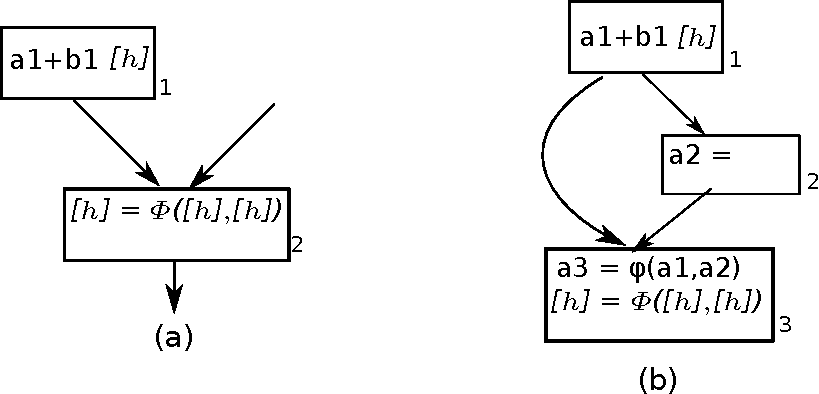
\includegraphics[scale=0.55]{fig-phi-insertion.pdf}
\caption{Examples of $\Phi$ insertion}
\label{fig: phi-insertion}
\end{figure}

\subsection{Step 2: Rename}

The Rename step assigns SSA versions to $h$ in its SSA form.  The version 
numbering produced for $h$ differs from the eventual SSA form for the 
temporary $t$, but has the following two important properties.  First,
occurrences that have idential $h$-versions have identical values.  Second,
any control flow path that includes two different $h$-versions must cross an
assignment to an operand of the expression of a $\Phi$ for $h$.

We conduct a preorder traversal of the dominator tree similar to the renaming
step in SSA construction for variables, but with the following modification.
In addition to a renaming stack for each variable, we
maintain a renaming stack for the expression. Entries on the expression
stack are popped as our dominator tree traversal backtracks past the
blocks that contain them.  Maintaining the variable and expression stacks
together allows us to decide efficiently whether two occurrences of an
expression should be given the same $h$-version.

There are three kinds of occurrences of expressions in the program:
(1) the occurrences in the original program, which we call \emph{real}
occurrences; (2) the $\Phi$'s inserted in the $\Phi$-Insertion step; and
(3) $\Phi$ operands, which are regarded as occurring at the ends of the
predecessor blocks of the corresponding edges.  The Rename algorithm
performs the following steps upon encountering an occurrence $q$ of the
expression.  If $q$ is a $\Phi$, it is given a new $h$-version.  Otherwise,
we check the current version of every variable in the expression (i.e. the
version on the top of each variable's rename stack) against the version of
the corresponding variable in the occurrence on the top of the expression's
rename stack.  If all the variable versions match, we assign $q$ the same
$h$-version as the top of the expression's rename stack.  If any of the 
variable versions does not match, we have two cases: (a) if $q$ is a real
occurrence, we assign $q$ a new $h$-version; (b) if $q$ is a $\Phi$ operand,
we assign the special class $\bot$ to that $\Phi$ operand to denote that
the value of the expression is unavailable at that point.  These two
situations are illustrated in Figure~\ref{fig: rename}.  Finally, we push
$q$ on the expression stack and proceed.

\begin{figure}
\centering
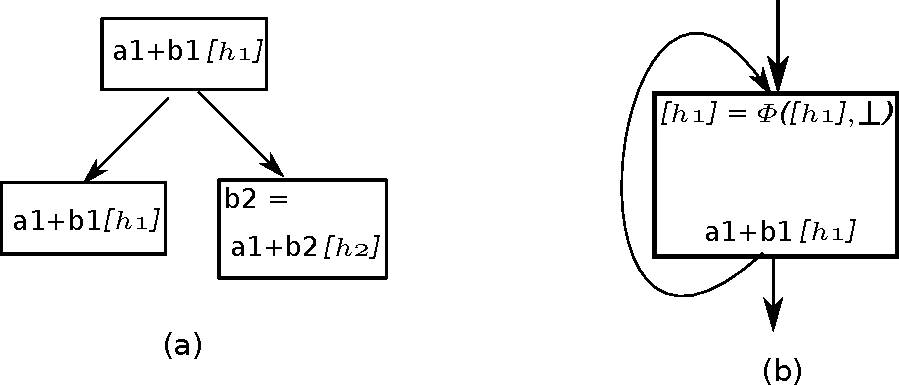
\includegraphics[scale=0.55]{fig-rename.pdf}
\caption{Examples of expression renaming}
\label{fig: rename}
\end{figure}

\subsection{Step 3: DownSafety}

The purpose of the DownSafety step is to satisfy the first requirement
that we discussed in 
Section~\ref{section:Part3:Pre_not_helped:PRErelatedtoSSA}
that any inserted computation must be safe.  This means that a computation
can only be inserted at a $\Phi$ where the computation is down-safe (or
anticipated).  Using the SSA graph, down-safety can be sparesely computed
by backward propagation along the use-def edges.

A $\Phi$ is not down-safe if there is a control flow path from that $\Phi$
along which the expression is not evaluated before program exit or before 
being altered by redefinition of one of its variables.  Except for loops with
no exit, this can happen only due to one of the following cases: (a) there
is a path to exit along which the $\Phi$ result version is not used; or (b)
there is a path to exit along which the only use of the $\Phi$ result
version is as an operand of a $\Phi$ that is not down-safe.  Case (a)
represents the initialization for our backward propagation of down-safety;
all other $\Phi$'s are initially marked \emph{downsafe}.  Down-safety
propagation is based on case (b).  Since a real occurrence of the
expression blocks the case (b) propagation, the algorithm marks each
$\Phi$ operand with a flag \emph{has\_real\_use} when the path to the $\Phi$
operand crosses a real occurrence of the same version of the expression.
Figure~\ref{fig: downsafety} gives the DownSafety propagation algorithm.

\begin{figure}[!ht]
{\bf procedure} Reset\_downsafe($X$) 
\{
\begin{code}
\x1 {\bf if} ($has\_real\_use(X)$ {\bf or} $def(X)$ is not a $\Phi$)
\x2   {\bf return}
\x1 $f \leftarrow def(X)$
\x1 {\bf if} ({\bf not} $downsafe(f)$)
\x2   {\bf return}
\x1 $downsafe(f) \leftarrow$ false
\x1 {\bf for} each operand $\omega$ of $f$ {\bf do}
\x2   Reset\_downsafe($\omega$)
\end{code}
\}

{\bf procedure} DownSafety
\{
\begin{code}
\x1 {\bf for} each $f \in$ \{$\Phi$'s in the program\} {\bf do}
\x2   {\bf if} ({\bf not} downsafe($f$))
\x3     {\bf for} each operand $\omega$ of $f$ {\bf do}
\x4	  Reset\_downsafe($\omega$)
\end{code}
\}
\caption{Algorithm for DownSafety}
\label{fig: downsafety}
\end{figure}

\subsection{Step 4: WillBeAvail}

The WillBeAvail step has the task of predicting whether the expression
will be available at each $\Phi$ result following insertions for PRE.
In the Finalize step, insertions will be performed at incoming edges
corresponding to $\Phi$ operands at which the expression will not be
available (without that insertion), but the $\Phi$'s \emph{will\_be\_avail} 
predicate is true.

The WillBeAvail step consists of two forward propagation passes performed
sequentially.  The purpose of the first forward propagation pass is to 
satisfy the second requirement that we discussed in 
Section~\ref{section:Part3:Pre_not_helped:PRErelatedtoSSA}
that the placements be computationally optimal.   This is done by computing
the \emph{can\_be\_avail} predicate, which gives possible points for
insertion for computational optimality  This predicate is first initialized
to true for all $\Phi$'s.  It then begins with the "boundary" set of $\Phi$'s
at which the expression cannot be made available by any downsafe set of
insertions.  These are $\Phi$'s that do not satisfy the \emph{downsafe}
predicate and have at least one $\bot$-valued operand.  The 
\emph{can\_be\_avail} predicate is set to false and the false value is
propagated from such nodes to others that are not downsafe and that are
reachable along def-use arcs in the SSA graph, excluding arcs at which
\emph{has\_real\_use} is true.  $\Phi$ operands defined by $\Phi$'s that
are not \emph{can\_be\_avail} are set to $\bot$ along the way.  After this
propagation step, \emph{can\_be\_avail} is false for a $\Phi$ if and only if
no downsafe placement of computations can make the expression available.
Figure~\ref{fig: canbeavail} gives the propagation algorithm for
\emph{can\_be\_avail}.

\begin{figure}[!ht]
{\bf procedure} Reset\_can\_be\_avail($g$) 
\{
\begin{code}
\x1 $can\_be\_avail(g) \leftarrow$ false
\x1 {\bf for} each $f \in$ \{$\Phi$'s with operand $\omega$ where $def(\omega) = g$\} {\bf do}
\x2   {\bf if} ({\bf not} $has\_real\_use(\omega)$)
\x3     {\bf if} ({\bf not} $downsafe(f)$ {\bf and} $can\_be\_avail(f)$)
\x4       Reset\_can\_be\_avail($f$)
\end{code}
\}

{\bf procedure} Compute\_can\_be\_avail
\{
\begin{code}
\x1 {\bf for} each $f \in$ \{$\Phi$'s in the program\} {\bf do}
\x2   $can\_be\_avail(f) \leftarrow$ true
\x1 {\bf for} each $f \in$ \{$\Phi$'s in the program\} {\bf do}
\x2   {\bf if} ({\bf not} $downsafe(f)$ {\bf and}
\x3       $can\_be\_avail(f)$ {\bf and}
\x3       $\exists$ an operand of $f$ that is $\bot$)
\x4	Reset\_can\_be\_avail($f$)
\end{code}
\}
\caption{Algorithm for \emph{can\_be\_avail}}
\label{fig: canbeavail}
\end{figure}

The purpose of the second forward propagation pass is to 
satisfy the third requirement that we discussed in 
Section~\ref{section:Part3:Pre_not_helped:PRErelatedtoSSA}
that the temporaries introduced to store the computation for reuse be 
lifetime optimal. The second pass works within the region computed by the
first pass to determine the \emph{later} attribute. 
A true value for this \emph{later} attribute means that the insertion
can be postponed.  This
is analogous to the computation of the predicate LATERIN
in Drechsler and Stade\cite{DS93}.  The \emph{later}
predicate is initialized to true wherever \emph{can\_be\_avail} is
true.  It then begins with the $\Phi$ operands corresponding to real
occurrences of the expressions in the program, and propagates the false value
for \emph{later} forward to those $\Phi$'s beyond which insertions cannot be
postponed (moved downward) without introducing unnecessary new 
redundancy\footnote{The result is that those $\Phi$'s satisfying \emph{later}
are exactly those that are \emph{can\_be\_avail} but not reachable from
any real occurrence along any forward arcs in the SSA graph.}
\emph{can\_be\_avail} $\Phi$'s marked not-\emph{later} are then the $\Phi$'s
where insertion should be performed for lifetime optimality in the introduced
temporary.   Thus, at the end of this second pass, \emph{will\_be\_avail}
for a $\Phi$ is given by $$will\_be\_avail = can\_be\_avail\ \wedge\ \urcorner later.$$
Figure~\ref{fig: later} gives the propagation algorithm for \emph{later}.

\begin{figure}[!ht]
{\bf procedure} Reset\_later($g$) 
\{
\begin{code}
\x1 $later(g) \leftarrow$ false
\x1 {\bf for} each $f \in$ \{$\Phi$'s with operand $\omega$ where $def(\omega) = g$\} {\bf do}
\x2   {\bf if} ($later(f)$)
\x3       Reset\_later($f$)
\end{code}
\}

{\bf procedure} Compute\_later
\{
\begin{code}
\x1 {\bf for} each $f \in$ \{$\Phi$'s in the program\} {\bf do}
\x2   $later(f) \leftarrow can\_be\_avail(f)$
\x1 {\bf for} each $f \in$ \{$\Phi$'s in the program\} {\bf do}
\x2   {\bf if} ($later(f)$ {\bf and}
\x3       $\exists$ an operand $\omega$ of $f$ such that ($def(\omega) \neq \bot$ {\bf and} $has\_real\_use(\omega)$))
\x4	Reset\_later($f$)
\end{code}
\}
\caption{Algorithm for \emph{later}}
\label{fig: later}
\end{figure}

We define the predicate \emph{insert} to indicate those $\Phi$ operands
where we will perform insertions.  \emph{insert} holds for a $\Phi$ operand
if and only if the following hold:

\begin{itemize}
\item the $\Phi$ satisfies \emph{will\_be\_avail}; and
\item the operand is $\bot$; or \emph{has\_real\_use} is false for the
operand and the operand is defined by a $\Phi$ that does not satisfy
\em{will\_be\_avail}.
\end{itemize}

\subsection{Step 5: Finalize}

The SSA graph built for the expression is mainly data flow analysis purpose.
At this point, the placement problem has been solved, and it is time to
transform the program.
The Finalize step plays the role of transforming the SSA graph for the
hypothetical temporary $h$ to the valid SSA form that reflects insertions 
and in which no $\Phi$ operand is $\bot$.  The Finalize step consists of
two parts, Finalize\_1 and Finalize\_2.  Finalize\_1 performs the
following tasks:

\begin{itemize}
\item For each real occurrence of the expression, it marks it with a $reload$
flag to indicate whether it should be computed on the spot or reloaded
from the temporary.
\item For $\Phi$'s where \emph{will\_be\_avail} is true, insertions are
performed at the incoming edges that correspond to $\Phi$ operands at which
the expression is not available.
\item $\Phi$'s whose \emph{will\_be\_avail} predicate is true may become
$\phi$'s for $t$.  $\Phi$'s that are not \emph{will\_be\_avail} will not
be part of the SSA form for $t$, and arcs from \emph{will\_be\_avail} 
$\Phi$'s that reference them are fixed up to refer to other (real or 
inserted) occurrences.
\item The SSA graph is updated to reflect the factored use-def relation
for the expression temporary.  This restructuring is accomplished by
resetting the $def$ field of each operand of a $\Phi$ satisfying
\emph{will\_be\_avail} and each real occurrence that will be reloaded so
that these $def$ fields refer to the expression occurrences that will be
their definitions in the final SSA form of the temporary.
\end{itemize}

Finalize\_2 performs the following two tasks:

\begin{itemize}
\item For each real occurrence that is not reloaded, it marks it with a
$save$ flag to indicate whether the computed value should be saved to the 
temporary.
\item Extraneous $\Phi$'s are removed.
\end{itemize}

Finalize\_1 is performed via a preorder traversal of the dominator tree
of the program control flow graph.  Though modeled after the rename step
in SSA construction, Finalize\_1 does not require any renaming stack for
its operation, because SSA versions have already been assigned.  Instead,
it sets up a table $Avail\_def$ (for \emph{available definitions}) to do its
job, which incurs less overhead than the stack operation, with the indices
into the table being the $h$-version number.  $Avail\_def$[x] will point
to the expression occurrence that defines that $h$-version, with the
defining occurrence being either (a) a real occurrence or (b) a $\Phi$ for
which \emph{will\_be\_avail} is true.  The algorithm for Finalize\_1 is
given in Figure~\ref{fig: finalize1}.

\begin{figure}[!ht]
{\bf procedure} Finalize\_1
\{
\begin{code}
\x1 $Avail\_def[] \leftarrow \bot$
\x1 {\bf for} each occurrence $X$ in preorder dominator tree traversal order {\bf do} \{
\x2   $x \leftarrow h\_version(X)$
\x2   {\bf if} ($X$ is a $\Phi$ occurrence) \{
\x3	{\bf if} ($will\_be\_avail(f)$)
\x4	  $Avail\_def[x] \leftarrow f$
\x2   \}
\x2   {\bf else if} ($X$ is a real occurrence) \{
\x3	{\bf if} ($Avail\_def[x]$ is $\bot$ {\bf or} $Avail\_def[x]$ does not dominate $X$) \{
\x4	  $reload(X) \leftarrow$ false
\x4	  $Avail\_def[x] \leftarrow X$
\x3	\}
\x3	{\bf else} \{
\x4	  $reload(X) \leftarrow$ true
\x4	  $def(X) \leftarrow Avail\_def[x]$
\x3	\}
\x2   \}
\x2   {\bf else} \{ /* $X$ is a $\Phi$ operand occurrence */
\x3     let $f$ be the $\Phi$ in the successor block of this operand
\x3	{\bf if} ($will\_be\_avail(f)$)
\x4	  {\bf if} ($X$ satisfies $insert$) \{
\x5	    insert the current expression at the end of the block containing $X$
\x5	    $def(X) \leftarrow$ inserted occurrence
\x4	  \}
\x4	  {\bf else}
\x5	    $def(X) \leftarrow Avail\_def[x]$
\x2   \}
\x1 \}
\end{code}
\}
\caption{Algorithm for Finalize\_1}
\label{fig: finalize1}
\end{figure}

To determine those real occurrences that must be saved to the temporary,
Finalize\_2 performs a backward search over the SSA graph.  The search
begins at the set of real occurrences that are marked $reload$ and progresses
backward along upward arcs using the $def$ field for each reloaded real
occurrence as set by Finalize\_1.  Every real occurrence that defines a
$\Phi$ operand or real occurrence encountered in the search will have its
$save$ flag set.

$\Phi$'s can be determined to be extraneous by SSA minimization modeled
after the $\phi$ insertion step in SSA construction. We initially mark
all the $\Phi$'s as being extraneous.  Base on the iterated dominance
frontier of the set of real occurrences with the $save$ flag set plus
the inserted computations, we can find and mark the $\Phi$'s that are not
extraneous.
Removing an extraneous $\Phi$ requires changing the occurrences assigned
the $h$-version of the extraneous $\Phi$ to a different one.  The replacing
$h$-version can be found by tracing up the $\Phi$ operands  This process
is integrated into the Finalize\_2 pass given in Figure~\ref{fig: finalize2}.

\begin{figure}[!ht]
{\bf procedure} Set\_save($X$) 
\{
\begin{code}
\x1 {\bf if} ($X$ is a real occurrence)
\x2   $save(X) \leftarrow$ true
\x1 {\bf else if} ($X$ is a $\Phi$ occurrence)
\x2   {\bf for} each operand $\omega$ of $X$ {\bf do}
\x3	{\bf if} ({\bf not} $processed(\omega)$)
\x4       Set\_save($def(\omega)$)
\x1 {\bf if} ($X$ is real or inserted)
\x2   {\bf for} each $f \in F$ marked $will\_be\_avail$ appearing in $DF^+(X)$ {\bf do}
\x3       $extraneous(f) \leftarrow$ false
\end{code}
\}

{\bf procedure} Set\_replacement($g$, $replacing\_def$)
\{
\begin{code}
\x1 {\bf for} each $will\_be\_avail f \in F$ with $j$th operand defined by $g$\} {\bf do}
\x2   {\bf if} ($extraneous(f)$)
\x3	Set\_replacement($f$,$replacing\_def$)
\x2   {\bf else}
\x3	replace $j$th operand of $f$ by $replacing\_def$
\x1 {\bf for} each real occurrence $X$ satisfying $reload$ with $def(X) = g$ {\bf do}
\x2   $def(X) \leftarrow replacing\_def$
\x1 $F \leftarrow F - \{g\}$
\end{code}
\}

{\bf procedure} Finalize\_2
\{
\begin{code}
\x1 $F \leftarrow$ \{$\Phi$'s in the program\}
\x1 {\bf for} each $f \in F$ satisfying $will\_be\_avail$ {\bf do}
\x2   $extraneous(f) \leftarrow$ true
\x1 {\bf for} each real occurrence $X$ {\bf do}
\x2   $save(X) \leftarrow$ false
\x1 {\bf for} each $f \in F$ {\bf do}
\x2   {\bf for} each operand $\omega$ of $f$ {\bf do} 
\x3     $processed(\omega) \leftarrow$ false
\x1 {\bf for} each real occurrence $X$ satisfying $reload$ {\bf do}
\x2   Set\_save($def(X)$)
\x1 {\bf for} each $f \in F$ {\bf do}
\x2   {\bf if} $f$ satisfies $will\_be\_avail$ \{
\x3	{\bf if} ($extraneous(f)$)
\x4	  {\bf for} each operand $\omega$ of $f$ {\bf do}
\x5	    {\bf if} (($def(\omega)$ is a $\Phi$ {\bf and not} $extraneous(def(\omega))$) {\bf or}
\x6	      ($def(\omega)$ is real) {\bf or}
\x6	      ($def(\omega)$ is inserted))
\x7		Set\_replacement($f$,$def(\omega)$)
\x2   \}
\x2   {\bf else}
\x3	$F \leftarrow F - \{f\}$
\end{code}
\}
\caption{Algorithm for Finalize\_2}
\label{fig: finalize2}
\end{figure}

\subsection{Step 6: CodeMotion}

Once the hypothetical temporary $h$ has been put into valid SSA form, the
only remaining task is to update the native SSA program representation to
reflect the results of PRE.  This involves introducing the expression
temporary $t$.

The CodeMotion step walks over the SSA graph of $h$ in dominator-tree 
preorder.  At a real occurrence, if $save$ is true, it generates a save
of the result of the computation into a new version of $t$.  For $\Phi$
operand occurrences and real occurrences with the $reload$ flag set, it
replaces the computation by a use of $t$.  At an inserted occurrence, it
saves the value of the inserted computation into a new version of $t$.
At a $\Phi$ of $h$, it generates a corresponding $\phi$ for $t$.

\section{Practical Implementation of SSAPRE}

In this section, we discuss the practical aspects of applying SSAPRE to 
all the expression candidates in a function.

\subsection{Worklist-Driven PRE}

Since PRE work on the global scope, each lexically identified expression in
the program is a candidate for PRE.  Due to its sparse approach, SSAPRE 
is more suited to working on one expression at a time.   This also reduces
the memory requirement while applying the algorithm, because the intermediate
data structures for processing the expressions do not have to co-exist.

The lexically identified expressions that need to be worked on by SSAPRE
are managed in a worklist.  This is created in an initial pass, called
Collect-Occurrences, that scans the function to collect these expressions.
Collect-Occurrences is the only pass that needs to look at the entire
function.  For each lexically identified expression, we represent its
occurrences in the program by a set of \emph{occurrence nodes}.  Each
occurrence node provides enough information to pinpoint the location of that
occurrence in the function.  The six steps of SSAPRE operate on each
lexically identified expression based only on its occurrence nodes.

The occurrence nodes created by Collect-Occurrences are called \emph{real}
occurrence nodes, because they correspond to occurrences of the expression in
the input program.  There are other kinds of occurrence nodes represented
during the six steps of SSAPRE.  Based on the real occurrence ndoes,
$\Phi$-Insertion creates $\Phi$ occurrence nodes.  From the $\Phi$ occurrence
nodes, it also creates $\Phi$-predecessor occurrence nodes, one at the end
of each block that is a predecessor of some block containing a $\Phi$.
$\Phi$-predecessor occurrences serve as placeholders for $\Phi$ operands, as
the operands are regarded as occurring at the predecessors of the block
containing the $\Phi$.

To represent the SSA graph of the expression, each occurrence node has a field
for storing the $h$-version number assigned to it.  For a $\Phi$-predecessor
node or a real occurrence node that represents a use, the \emph{def} field
points to the representative occurrence for the $h$-version.  For $\Phi$
occurrence nodes, the $\Phi$ operands and result are provided.

Separately, there are \emph{exit} occurrence nodes for indicating when we
reach a point of program exit.  They are used only in the Rename step for
initializing the $downsafe$ flag.

In the remaining steps of SSAPRE, we need to visit the occurrence nodes in an
order corresponding to a preorder traversal of the dominator tree (DT) of the
control flow graph.  To facilitate this, we maintain the sequence of
occurrence nodes in this sorted order.  We precompute the 
\emph{depth-first-number} (\emph{dfn}) and the number of descendents
(\emph{des}) for each node in the DT.  For any two basic blocks $x$ and $y$,
we can determine whether $x$ dominates $y$ using the formula
$$Dominate(x,y) \equiv dfn(x) \leq dfn(y) \leq dfn(x) + des(x).$$
When we walk through the sequence of basic blocks in dominator-tree preorder,
a true value for $Dominate(x,y)$ indicates that we are descending the DT.
A false value for
$Dominate(x,y)$ alerts us to the need to take appropriate action due
to the fact that we are backtracking up the DT; in the case of Rename, it is
necessary to pop the renaming stack until the version at the top of the stack
is defined at a block that dominates $y$.  These observations allow us to walk
the occurrence list in dominator-tree preorder without a recursive descent of
the dominator tree.

\subsection{Nested Expressions}

PRE is applicable to any expressions whether it be simple, like $a+b$, or
compound, like $(a+b)-c$.  By working on one expression at a time, it is 
possible to exploit the nesting relationships
between expressions to achieve an overall speedup in SSAPRE.  This is based
on the following observation:
\begin{quote}
If redundancy exists in a compound expression, the same redundancy exists in
all the operators within the expression.  Conversely, if a simple expression
does not exhibit any redundancy, no compound expression that contains that
simple expression exhibits redundancy.
\end{quote}
For example, if redundancy exists for $(a+b)-c$, the same redundancy must
exist for $a+b$.  If $a+b$ does not exhibit redundancy, then $(a+b)-c$ also
must not exhibit redundancy.  If $a+b$ has redundancy, however, no inference
can be drawn regarding redundancy for the $-$ operation in $(a+b)-c$.

Elimination of redundancy always results in converting the expression to a
temporary, so the above observation leads to a strategy for dealing with
the optimization of compound expressions.  The strategy is to defer PRE for
compound expressions until they become converted to simple expressions by
PRE of their constituent expressions.  In our worklist-driven approach,
this implies that only simple expressions are allowed in the worklist.
As their optimizations proceed, some simple expressions will be converted to
temporaries, which in turn causes some compound expressions to become
simple expressions.  As new simple expressions are formed, they are entered
into the worklist.

As an example, for $(a+b)-c$, $a+b$ is first entered into the worklist by
Collect-Occurrences.  After SSAPRE has worked on $a+b$, any redundant occurrence
of $a+b$ will be replaced by a temporary $t$.  If PRE on $a+b$ converts
$(a+b)-c$ to $t-c$, this new simple expression, formed in the CodeMotion step,
will be entered as a new member of the worklist.  Redundancies of $t-c$, and
hence redundancies in $(a+b)-c$, will be eliminated later when SSAPRE
processes $t-c$.  If the expression $(a+b)-c$ does not yield $t-c$ when $a+b$
is processed, $(a+b)-c$ will remain a compound expression and will never need
to be processed by SSAPRE.

\begin{figure}
\centering
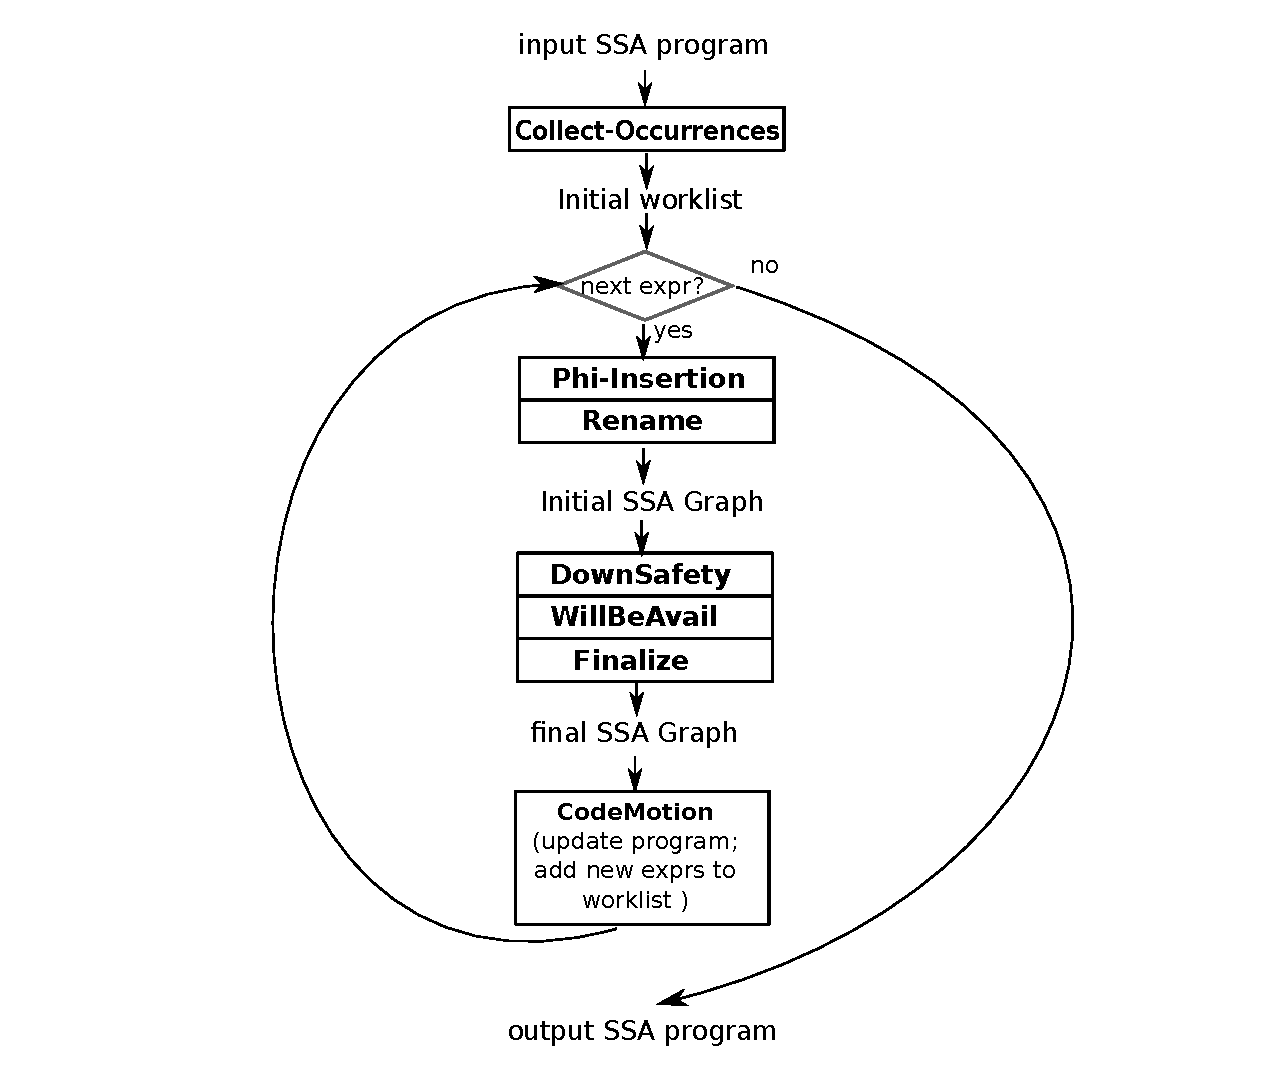
\includegraphics[scale=0.45]{fig-ssapre-flow.pdf}
\caption{SSAPRE processing flow chart}
\label{fig: ssapre-flow}
\end{figure}

In the absence of redundancy, SSAPRE terminates quickly because it can skip
the processing of all compound expressions.  In the presence of redundancies,
the approach has the secondary effect of converting the evaluation of compound
expressions essentially to triplet form, because the result of each simple
expression is saved to a temporary, which is then used as an operand in the
evaluation of another simple expression.  If this effect is undesirable,
the compound expressions can be re-constructed by performing copy propagation
on the temporaries that have only one locally occurring use.  After copy
propagation, the temporaries can be eliminated by dead-store elimination.  But
in the usual case the program will eventually be translated to machine
instructions, so the triplet form poses no obstacle for most target 
architectures.  Figure~\ref{fig: ssapre-flow} shows the flow chart of an
implementation of SSAPRE based on worklists that incorporates the above
strategy of dealing with compound expressions.
 
\section{Speculative PRE}

Speculative code motion ignores the safety requirement of PRE that we
discussed in Section~\ref{section:Part3:Pre_not_helped:PRErelatedtoSSA}.
In the absence of systems support, speculation is only applicable to 
expressions that will not cause runtime exceptions or faults, since such
exceptions or faults will alter the external behavior of the program.  
For example, indirect loads from unknown pointer values cannot be speculated
unless the systems would mask out the effect of loading from invalid addresses.
Speculative code motion suppresses
redundancy in some path at the expense of another path where the computation 
is added but result is unused.  As long as the path that is burdened with
more computations is executed less frequently than the path where the
redundant computations are avoided, a net gain in program performance can be
achieved.  Thus, speculative code motion should only be performed when there
are clues about the relative execution frequencies of the paths involved.

In SSAPRE, speculation corresponds to inserting computations at $\Phi$'s where
the computation is not downsafe.  This effect can be accomplished by 
marking those $\Phi$'s as downsafe in the DownSafety step.

Without profile data, speculative PRE can be conservatively performed by
restricting it to loop-invariant computations.  Figure~\ref{fig: spec-pre} shows
a loop-invariant computation $a+b$ that occurs in a branch inside the loop.
This loop-invariant code motion is speculative because, depending on the
branch condition inside the loop, it may be executed zero time, while moving it
to the loop header causes it to execute one time. This speculative 
loop-invariant code motion is generally profitable because the benefit of
suppressing its computation inside the loop outweighs the cost of computing it
once at the loop header.  Marking $\Phi$'s located at the start of loop bodies
downsafe will effect speculative loop invariant code motion\cite{Lo98}. 

\begin{figure}
\centering
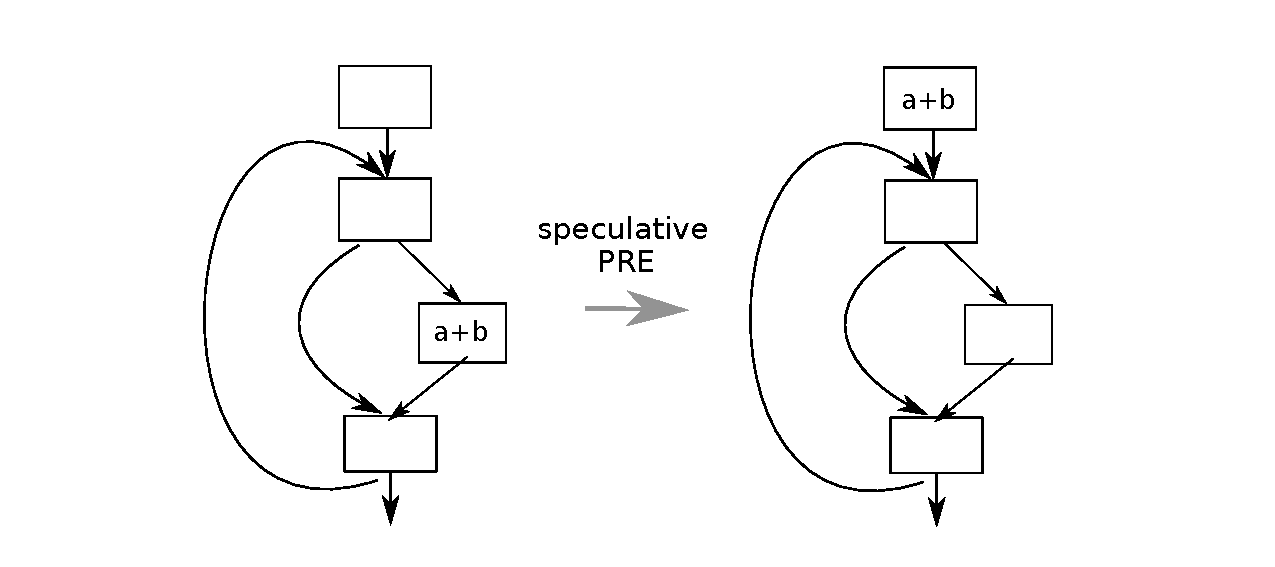
\includegraphics[scale=0.55]{fig-spec-pre.pdf}
\caption{Speculative loop-invariant code motion}
\label{fig: spec-pre}
\end{figure}

To enable more code motion of usually unsafe operations, Murphy {\it et al.} 
modify SSAPRE to use the fault safety property.   They define $dangerous$
computations as operations that may fault but will otherwise have no observable
side effects.  Such computations include indirect loads and divides.  Such
dangerous computations are sometimes protected by tests (or guards) placed in
the code by the programmers.  Compilers for languages like Java also insert 
runtime checks to ensure faults never occur. When such a test occur in the
program, the dangerous computation is said to be \emph{safety-dependent} on
the control flow point that establishes its safety.  A dangerous instruction
is \emph{fault-safe} at any point in the program where its safety dependence
is satisfied.

Murphy {\it et al.} represents safety dependences as value dependences in the
form of the abstract \emph{tau values} described in \cite{Menon06}.  Each check
that succeeds will define a tau value on its fall-through path.  During SSAPRE,
dangerous computations will have additional \emph{tau} operands attached to 
them.  The tau
operands are also variables in SSA form, so their definitions can
be found by following the use-def edges.  The compiler inserts the definitions
of the taus also with abstract right-hand-side values, like {\bf tauedge}.
Because they are abstract, they
are omitted in the generated code after the SSAPRE phase.  A dangerous
computation can be defined to have more than one tau operands, depending on
its semantics.  When all its tau operands have definitions, 
it means the computation is fault-safe; otherwise, it is unsafe.  
By including the tau operands into consideration, speculative PRE automatically
honors the fault-safety of dangerous computations when it performs speculative
code motion.

As an example, if we replace the expression $a+b$ in Figure~\ref{fig: spec-pre}
by $a/b$, the speculative code motion cannot be performed because if $b$ is 0,
the speculative insertion of $a/b$ at the loop header will cause a run-time
divide-by-zero fault.  In Figure~\ref{fig: spec-div}, the program contains a 
non-zero test for $b$.  We define a tau operand for $a/b$ in SSAPRE to
provide the information whether a non-zero test for b is available.  The
presense of the non-zero test for $b$ causes the compiler to insert the
definition of $tau1$ with the abstract right-hand-side value {\bf tauedge}.
Since the divide inside the loop $a_1/b_1,tau_1$ has a tau operand whose
definition is visible, speculative SSAPRE will force the $\Phi$ at the head
of the loop body to be downsafe.  When $a_1/b_1,tau_1$ is hoisted out of the
loop, it automatically stops at the definition of $tau_1$ because PRE obeys
value dependence.

\begin{figure}
\centering
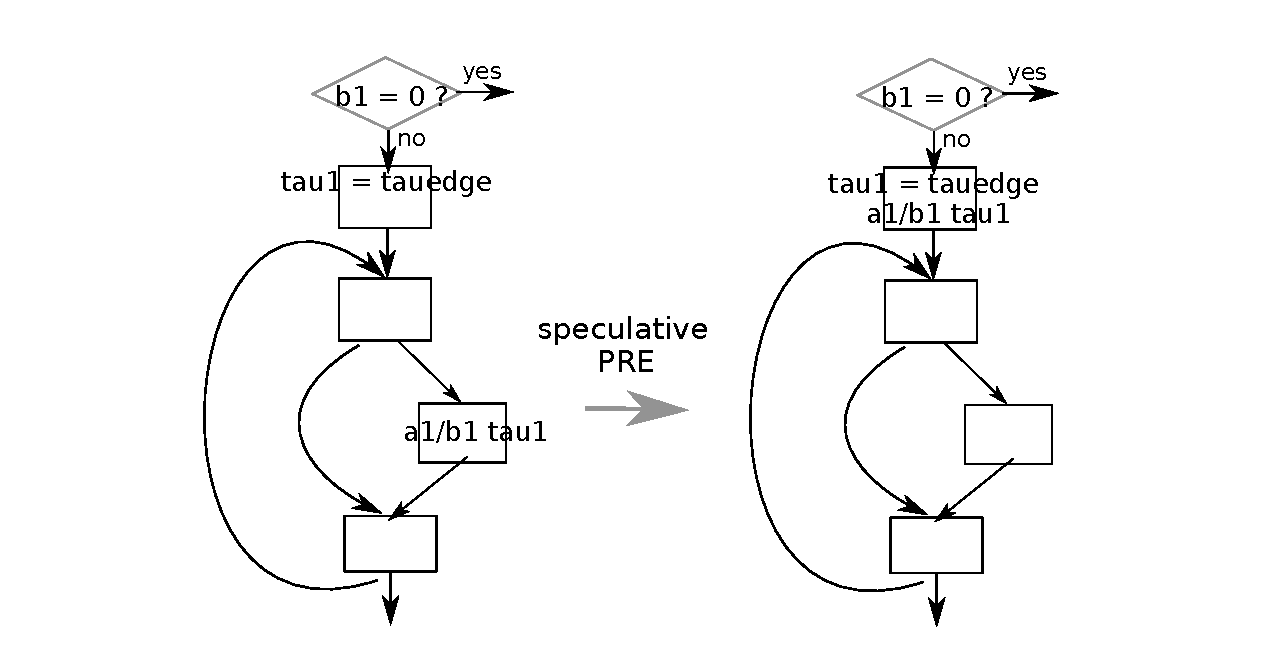
\includegraphics[scale=0.55]{fig-spec-div.pdf}
\caption{Speculative and fault-safe loop-invariant code motion}
\label{fig: spec-div}
\end{figure}

When execution profile data are available, it is possible to tailor the use
of speculation to maximize run-time performance for executions of the program
that match the profile.  An algorithm for profile-driven speculative SSAPRE
is described in \cite{Lo98}.  Xue and Cai present a computationally optimal
and lifetime optimal algorithm
for speculative PRE based on edge profile in \cite{Xue06}.  Their algorithm
uses bit-vector-based data flow analysis.

\section{Register Promotion via PRE}

Register promotion refers to the important task in an optimizing compiler
of identifying the data items that are candidates for register allocation 
in the program.  To represent register allocation candidates, compilers
commonly use an unlimited number of \emph{pseudo-registers}.  Pseudo-registers
are also called symbolic registers or virtual registers, to distinguish them
from real or physical registers.  Pseudo-registers have no alias, and the
process of assigning them to real registers involves only renaming them.

\subsection{Register Promotion as Placement Optimization}

Under PRE, the temporaries generated to hold the values of redundant 
computations are pseudo-registers.  Local variables determined by the compiler
to have no alias can be trivially renamed to pseudo-registers.   All remaining
register allocation candidates have to be assigned pseudo-registers through 
the process of register promotion.  Register promotion is also responsible
for generating the most efficient code to set up the data objects in
pseudo-registers.  Targets for register promotion include scalar variables,
indirectly accessd memory locations and program constants.  
Load operations are needed to put them into pseudo-registers before
they are used\footnote{Depending on the ISA, some constants may not need to be
put in registers, and they should be excluded from register promotion.}, and
when there is an assignment, a store operation is needed.  Since the goal of
register promotion is to obtain the most efficient placements for the loads and
stores, register promotion can be modeled as two separate problems: PRE of 
loads, followed by PRE of stores.

From the point of view of redundancy, loads are like expressions because the
later occurrences are the ones to be deleted.  For stores, the reverse is true:
the earlier stores are the ones to be deleted, as is evident in the examples
of Figure~\ref{fig: load-store-dual}(a) and (b).  The PRE of stores problem,
also called \emph{partial dead code elimination}, can thus be treated as the
dual of the PRE of loads problem.  Performing PRE of stores thus has the effects
of moving stores forward while inserting them as early as possible.  
Combining the effects of the PRE of loads and stores results in optimal
placements of loads and stores while minimizing the live ranges of the
pseudo-registers, by virtue of the computational and lifetime optimalities
of our PRE algorithm.

\begin{figure}
\centering
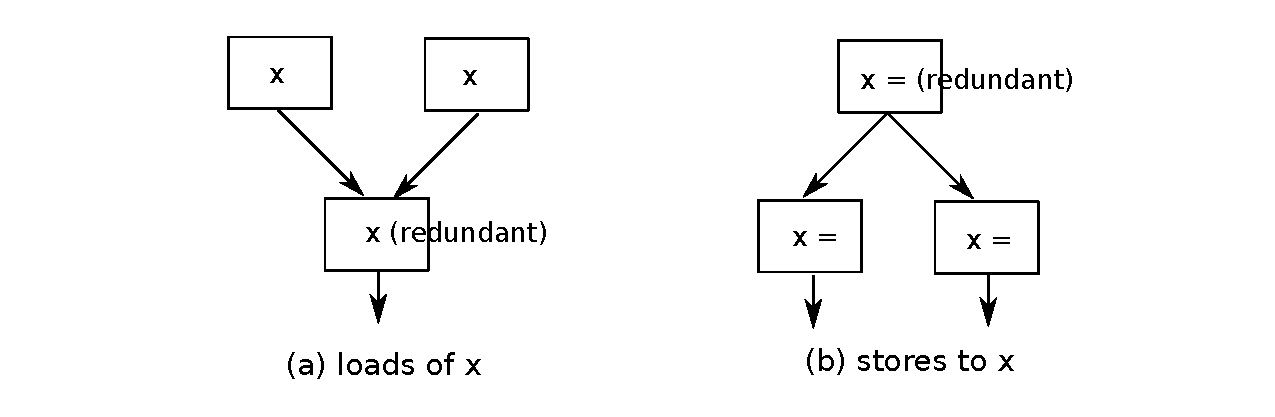
\includegraphics[scale=0.55]{fig-load-store-dual.pdf}
\caption{Duality between load and store redundancies}
\label{fig: load-store-dual}
\end{figure}

\subsection{Load Placement Optimization}

PRE applies to any computation including loads from memory locations and
loads of constants.  In program representations, loads can either be indirect 
through a pointer or direct.  Direct loads  and constants constitutes the leaves
in expression trees.  The bottom-up application of SSAPRE to an expression
tree will then start with the leaf nodes before the simple expressions.

When we apply SSAPRE to direct loads, since the hypothetical temporary $h$ can
be regarded as the candidate variable itself, the $\Phi$-insertion step and
Rename step can be streamlined.  In other words, the $\Phi$'s are the variable's
$\phi$'s, and the $h$-versions are the variable's SSA version.

When working on the PRE of memory loads, it is important to also take into
account the stores, which we call \emph{l-value} occurrences.  A store of the 
form $x \leftarrow \texttt{<expr>}$ can be regarded as being made up of the
sequence:
\begin{tabbing}
XX:\= while \= while \= while \= while \= while \= \kill

\> \> $r \leftarrow \texttt{<expr>}$ \\
\> \> $x \leftarrow r$ \\
\end{tabbing}
Because the pseudo-register $r$ contains the current value of $x$, any
subsequent occurrences of the load $x$ can reuse the value from $r$, and
thus can be regarded as redundant.   Figure~\ref{fig: lval-occur} gives examples
of loads made redundant by stores.

\begin{figure}
\centering
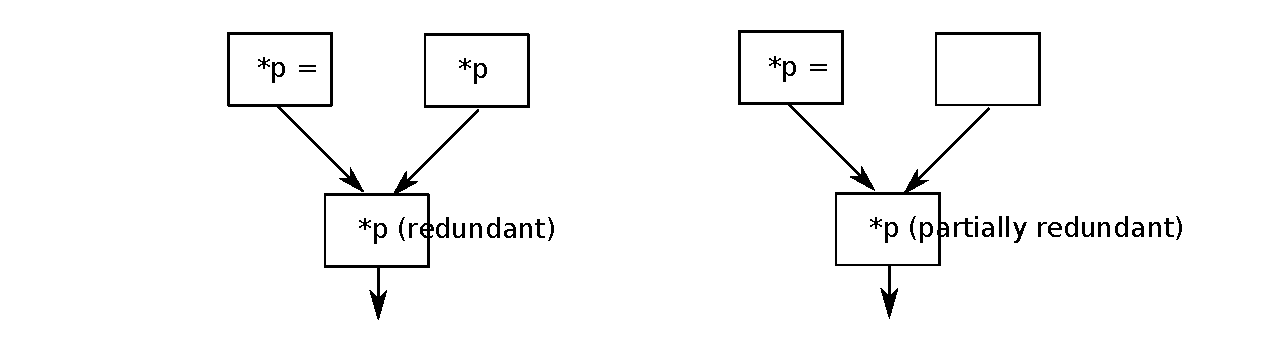
\includegraphics[scale=0.55]{fig-lval-occur}
\caption{Redundant loads after stores}
\label{fig: lval-occur}
\end{figure}

When we perform the PRE of loads, we thus include the l-value occurrences into
consideration.  The $\Phi$-insertion step will insert $\Phi$'s at the iterated
dominance frontiers of l-value occurrences.  In the Rename step, an l-value
occurrence is always given a new $h$-version, because a store is a definition.
Any subsequent load renamed to the same $h$-version is redundant with respect
to the store.

In the CodeMotion step, if an l-value occurrence is marked $save$, the
store statement $x \leftarrow \texttt{<expr>}$ will be split into two 
statements:
\begin{tabbing}
XX:\= while \= while \= while \= while \= while \= \kill

\> \> $t_1 \leftarrow \texttt{<expr>}$ \\
\> \> $x \leftarrow t_1$ \\
\end{tabbing}
The placement of the new store $x \leftarrow t_1$ will be optimized by the PRE
of stores performed later.

We apply the PRE of loads
first, followed by the PRE of stores.  This ordering is based on the fact that
the PRE of loads is not affected by the results of the PRE of stores, but the
PRE of loads creates more opportunities for the PRE of stores by deleting
loads that would otherwise have blocked the movement of stores.  In addition,
speculation is required for the PRE of loads and stores in order for register
promotion to do a decent job in loops.  

The example in Figure~\ref{fig: promotion-example} illustrates what we discuss
in this section.  During the PRE of loads (LPRE), $a =$ is regarded as an
l-value occurrence.  The hoisting of the load of $a$ to the loop header does
not involve speculation. The occurrence of $a =$ causes $r$ to be updated
by splitting the store into the two statements $r =$ followed by $a = r$.  In 
the PRE of stores (SPRE), speculation is needed to sink $a =$ to outside the
loop because the store occurs in a branch inside the loop.  Without performing 
LPRE first, the load of $a$ inside the loop would
have blocked the sinking of $a =$.

\begin{figure}
\centering
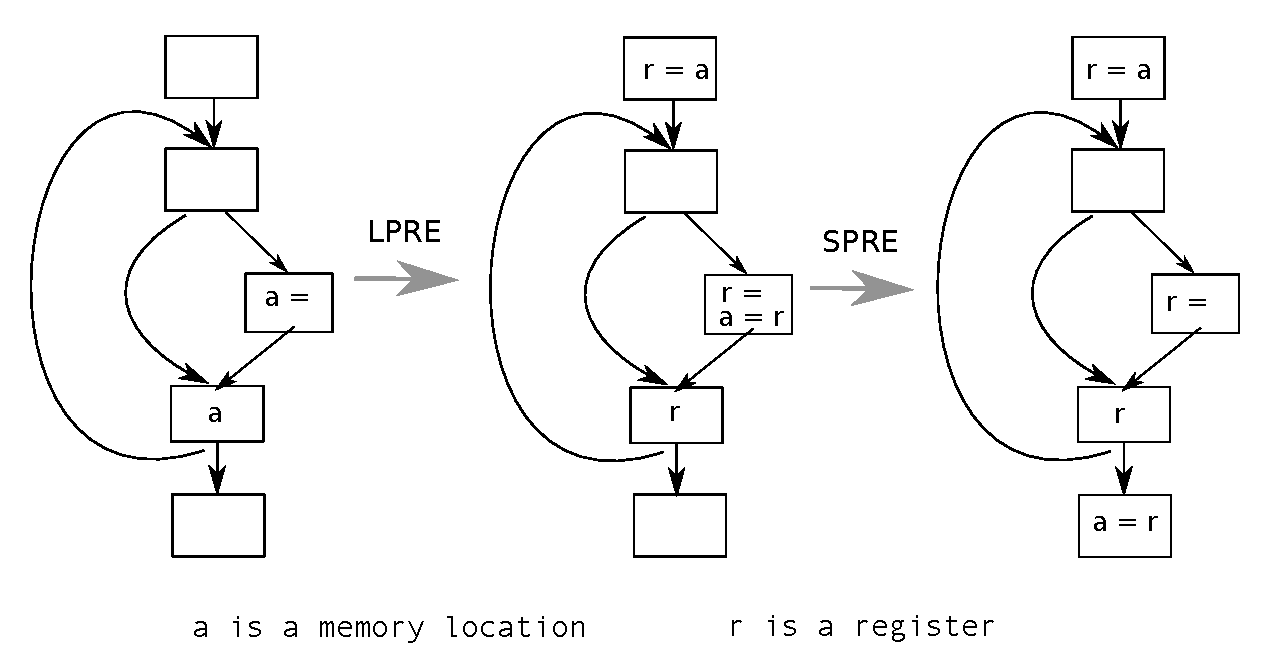
\includegraphics[scale=0.55]{fig-promotion-example.pdf}
\caption{Register promotion via load PRE followed by store PRE}
\label{fig: promotion-example}
\end{figure}

\subsection{Store Placement Optimization}

As mentioned earlier, the problem of SPRE is the dual of the problem of LPRE.
In the presence of store redundancies, the earlier occurrences are redundant.
Code motion in SPRE will have the effect of moving stores forward with respect 
to the control flow graph.  Presence of (aliased) loads have the effect of
blocking the movement of stores or rendering the earlier stores non-redundant.

To apply the dual of the SSAPRE algorithm, it is necessary to compute a program
representation that is the dual of the SSA form, and we call this the 
\emph{static single use} form.  In SSU, use-def edges are factored at
divergence points in the control flow graph.  We call this factoring operator
$\Lambda$.  Each use of a variable establishes a new version (we say the load 
\emph{uses} the version), and every store reaches exactly one load.   The
$\Lambda$ is regarded as a use of a new version of the variable.  The use
post-dominates all the stores of its version.  The left-hand-side of the
$\Lambda$ is the multiple definitions, each of which is post-dominated by their
single uses.

We call our store PRE algorithm SSUPRE, which is composed of the six steps
corresponding to SSAPRE.  The first two steps, $\Lambda$-Insertion and
SSU-Rename, create the SSU form for the variable.  The third step, UpSafety,
is just the reverse of DownSafety.  The fourth step, WillBeAnt, also corresponds
to WillBeAvail in reverse.  Though store elimination itself does not require
the introduction of temporaries, lifetime optimality still needs to be
considered for the temporaries introduced in the LPRE phase which hold the 
values to the point where the stores are placed.  Thus, it is desirable not 
to sink the stores too far down.  
The fifth and sixth step, Finalize and CodeMotion, is also simpler than 
SSAPRE because no temporary is introduced that needs to be put in SSA form.
However, for an inserted store, the variable will require a new SSA version,
and the later uses have to be updated to refer to the new store.
We add a post-pass to SSUPRE which is essentially the renaming step in SSA
construction to fix-up the use-defs due to the newly inserted stores.

\begin{figure}
\centering
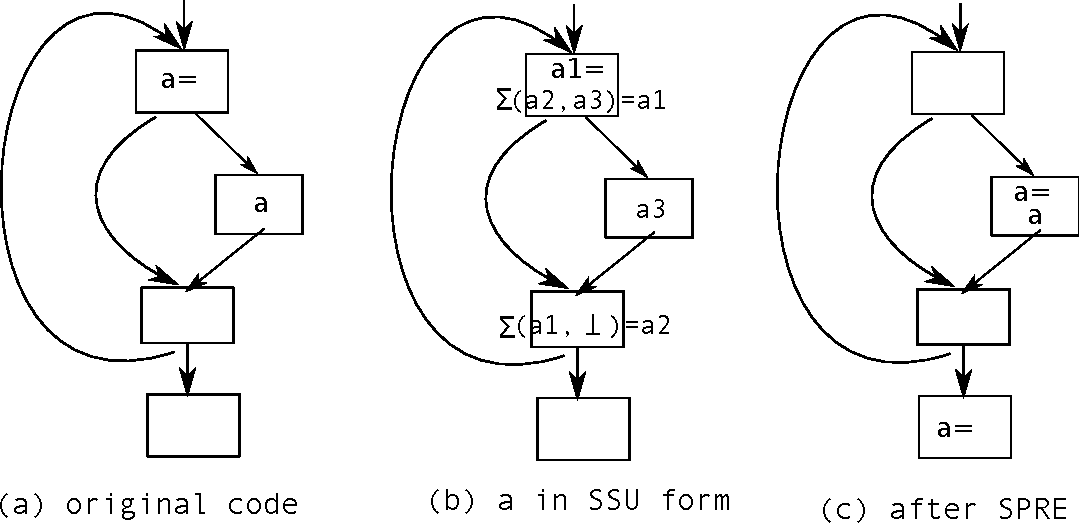
\includegraphics[scale=0.55]{fig-ssupre.pdf}
\caption{Example of program in SSU form and the result of applying SSUPRE}
\label{fig: ssupre}
\end{figure}

Figure~\ref{fig: ssupre} gives an example program with (b) being the SSU 
representation (a).  (c) shows the result of applying SSUPRE to the code.
The store can be sunk to outside the loop only if it is also inserted in
the branch inside the loop that contains the load.  The optimized code no
longer exhibits any store redundancy.

A limitation of the above SSUPRE algorithm is that it does not apply to 
indirect stores.  We think it is possible to extend the algorithm to make it
work on indirect stores as well.

\section{Redundancy via the Semantic Approach}
\label{section:Part3:Pre_not_helped:SemanticPRE}

The redundant computations stored into a temporary introduced by PRE may
be of different values because the same lexically identified expressions may
yield different results at different points in the program.
Since PRE applies only to lexically identified expressions, it is not capable
of recognizing redundant computations among lexically different expressions
based on their semantics.  On the other hand, under the semantic approach, 
redundant computations can be recognized among computations that are 
semantically determined to yield the same values.

\subsection{Value Numbering}

Computations are determined to yield the same value using \emph{value numbering}
analysis techniques.  The term \emph{value number} originated from the 
hash-based method developed by Cocke and Schwartz for recognizing when two
expressions evaluate to the same value within a basic block \cite{CS70}.  
The value number of an expression tree can be regarded as the index of its
hashed entry in the hash table.  
An expression tree is hashed bottom up starting with the leaf nodes.  
Each internal node is hashed based on its operator and the value numbers of 
its operands.  Two expressions with the same
value number \emph{must} evaluate to the same value at run-time.

When the program has been put into SSA form, value number can be extended to the
global scope by assigning a unique value number to each variable version by
virtue of the single definition property \cite{Rosen88}.  Additional 
refinements to hash-based global value numbering algorithms have been proposed
by Briggs {\it et al.} \cite{Briggs97}.

There is a second approach for determining whether two expressions compute the
same value that uses the partitioning method instead of hashing. 
First developed by
Alpern {\it et al.} \cite{AWZ88}, the algorithe partitions all the expressions
in the program into congruence classes.  Values in the same congruence class 
are considered equivalent.  The algorithm is optimistic because it
starts by putting all expressions based on the same operator into the same
congruence class.  As the algorithm iterates, it subdivides the congruence
classes into smaller ones, continuously increasing the number of congruence
classes.  The algorithm terminates when no more change occurs,
at which point an enumeration of the resultant congruence classes can be
used as value numbers.  This algorithm is shown in 
Figure~\ref{fig: partition-alg}. In the last {\bf for} loop, if $s$ is not in
the worklist (i.e. processed already), the partitioning was already stable 
with respect to $s$, and
we can add either $n$ or the shrunk $s$ to the worklist to re-stabilize with
respect to that split of $s$.  Choosing the smaller one results in less
overhead.

\begin{figure}[t]
\begin{center}
\fbox{ \parbox[t]{6.0in} {
\begin{tabbing}
XX:\= op \= op \= op \= op \= op \= \kill
Place all values computed by the same opcode in the same congruence class\\
$worklist \leftarrow$ set of all congruence classes\\
{\bf while} $worklist \neq \phi$ \\
\> Select and delete an arbitrary congruence class $c$ from $worklist$\\
\> {\bf for} each operand position $p$ of a use of $x \in c$\\
\>  \> $touched \leftarrow \phi$\\
\>  \> {\bf for} each $x \in c$\\
\>  \>  \> Add all uses of $x$ in position $p$ to $touched$\\
\>  \> {\bf for} each class $s$ such that $\phi \subset (s \cap touched) \subset s$\\
\>  \>  \> Create a new class $n \leftarrow s \cap tourhced$\\
\>  \>  \> $s \leftarrow s - n$\\
\>  \>  \> {\bf if} $s \in worklist$ \\
\>  \>  \>  \> Add $n$ to $worklist$ \\
\>  \>  \> {\bf else}\\
\>  \>  \>  \> Add smaller of $n$ and $s$ to $worklist$\\
\end{tabbing}}}
\caption{The partitioning algorithm}
\label{fig: partition-alg}
\end{center}
\end{figure}

There are also refinements to the partitioning technique described in
\cite{Briggs97}.  The partition-based algorithm does not supercede, but 
instead complements the hash-based algorithms.
The most powerful value numbering algorithms seem to be based on
a combination of the two approaches.

\subsection{Redundancy Elimination via Value Numbering}

So far, we have only talked about finding computations that compute the
same value, but have not addressed how to use the results of such analysis 
to optimize the program.  Two computations that compute the same value do
not necessarily exhibit redundancy if they are not situated on the same
execution path.  Thus, it is logical to consider performing PRE separately
to each value number.  

If we consider the temporary $t$ that will be introduced to store the redundant
computations under value-number-based PRE, we can see that its value will
stay the same throughout its lifetime.  If there are $\phi$'s introduced for
the temporary, they will be merging identical values, and we know from
experience that such $\phi$'s are rare.  A subset of such $\phi$'s is expected 
to come from PRE's insertions, and that implies that insertions
introduced by value-number-based PRE are also rare.

Value-number-based PRE also has to deal with the additional issue of \emph{how}
to generate an insertion.  Because the same value can come from different forms
of expressions at different points in the program, it is necessary to determine
which form to use at an insertion point.  If the insertion point is outside 
the live range of any variable version that can compute that value, then the
insertion point has to be disqualified.  Due to this complexity, and the
expectation that \emph{truly partial} redundancy is rare among computations
that yield the same value, we focus only on eliminating full redundancies
among computations that have the same value number\footnote{This assumes
PRE for lexically identified expressions have been applied, which would have
removed the redundancies among lexically identified expressions that also
have the same value number.}.

Since full redundancy elimination (FRE) is a subset of PRE, we can adapt the
SSAPRE algorithm to work on value-number-identified expressions and remove
full redundancies among them.  We call this adapted algorithm VNFRE.

In VNFRE, the $\Phi$-Insertion step only needs to consider the iterated
dominance frontiers.  It is not necessary to consider the variable operands,
because as long as the value number is the same, we do not have to consider
when any variable operand's value is changed. The Renaming step is also simpler
because we also ignore the variable operands.  In fact, the only situations 
where new $h$-versions are introduced are at program entry (when the renaming 
stack is empty) and when encountering $\Phi$'s.

The only data flow propagation needed under VNFRE is for the \emph{full 
availability}
attribute, which is the reverse of downsafety.  We initialize the $fully\_avail$
flag for each node in the SSA graph to $true$, except it is set to $false$ for
$\Phi$'s that have one or more $\bot$ operands.  The propagation step
propagates the $false$ value of $fully\_avail$ forward in the SSA graph.
We can reuse the algorithm of the Finalize step of SSAPRE after replacing 
$will\_be\_avail$ by $fully\_avail$, and setting $insert$ and
$later$ to $false$ for all nodes.

In practice, with copy propagation, constant folding and SSAPRE having been 
performed earlier, there are not much optimization opportunities left 
for VNFRE to cater to.  One useful application of VNFRE is in induction
variable collescing.  Code like the following, with multiple induction
variables, could be the result of
earlier optimizations like strength reduction:
{\tt
\begin{verbatim}
        i = 0;
        j = 0;
        while <cond> {
          i = i + 4;
          j = j + 4;
        }
\end{verbatim}
}

Value numbering will determine that at different points in the code, {\tt i}
and {\tt j} always have the same value number.  Performing VNFRE can yield the
net effect of getting rid of the extra induction variables.

\section{Conclusion}

The close relationsihp between PRE and SSA arises because 
partial redundancies can be exposed by factoring at control flow merge points.
The SSAPRE algorithm capitalizes on prior techniques developed for computing 
and manipulating SSA form.  The SSAPRE framework also shows that the 
concept and techniques of SSA can be made to apply to any program constructs, 
not just variables.  The constructed SSA graphs can then be used to 
efficiently perform sparse data flow propagation.

There are additional optimizations that can be implemented using the SSAPRE
framework that we have not covered.  They include code hoisting, register 
shrink-wrapping \cite{Chow88} and live range shrinking.  Moreover, PRE has 
traditionally provided the context for integrating additional optimizations 
into its framework.  They include operator strength reduction \cite{Knoop93} 
and linear function test replacement \cite{Kennedy98}.  As a result, PRE 
has become the most powerful and encompassing optimization framework in modern 
optimizing compilers.
